\section{Arquitectura General del Sistema}
El sistema adopta el paradigma de arquitectura de microservicios distribuidos, separando la lógica de presentación, la capa de persistencia/autorización y el cómputo intensivo de Inteligencia Artificial. Esta separación garantiza escalabilidad horizontal y alta disponibilidad frente a concurrencia estudiantil \cite{charland_mobile_2011, flutter_vs_ionic_2023}.

\subsection{Capa de Cliente (Frontend - SheetMusic Pedia)}
Desarrollada con Ionic React v8 y Capacitor v7, empaquetada como Progressive Web App (PWA) e instalable de forma nativa en dispositivos móviles. Utiliza React Query para la gestión del estado remoto y emite peticiones HTTPS/RESTful autenticadas mediante tokens JSON Web Tokens (JWT).

\subsection{Capa de Servicios de Backend (BaaS)}
Se utiliza Supabase sobre PostgreSQL 15, desplegado en la región AWS \textit{us-east-1} \cite{supabase_docs_2024}. Esta capa administra la identidad de los usuarios, almacena el historial de progreso y la telemetría académica, y aplica políticas de Row Level Security (RLS) para aislar la información entre roles (estudiantes y docentes). Toda comunicación con el cliente se realiza a través de procedimientos almacenados remotos (RPC) para minimizar los viajes de ida y vuelta a la red (\textit{round trips}).

\subsection{Capa de Inteligencia (Motor DRL)}
Construido sobre FastAPI, PyTorch y Stable-Baselines3 en Debian/Docker. Recibe el vector de estado del estudiante desde la API REST de backend, procesa las restricciones pedagógicas del árbol y devuelve en milisegundos la recomendación del siguiente ejercicio junto a su nivel de dificultad.

\begin{figure}[htbp]
\centerline{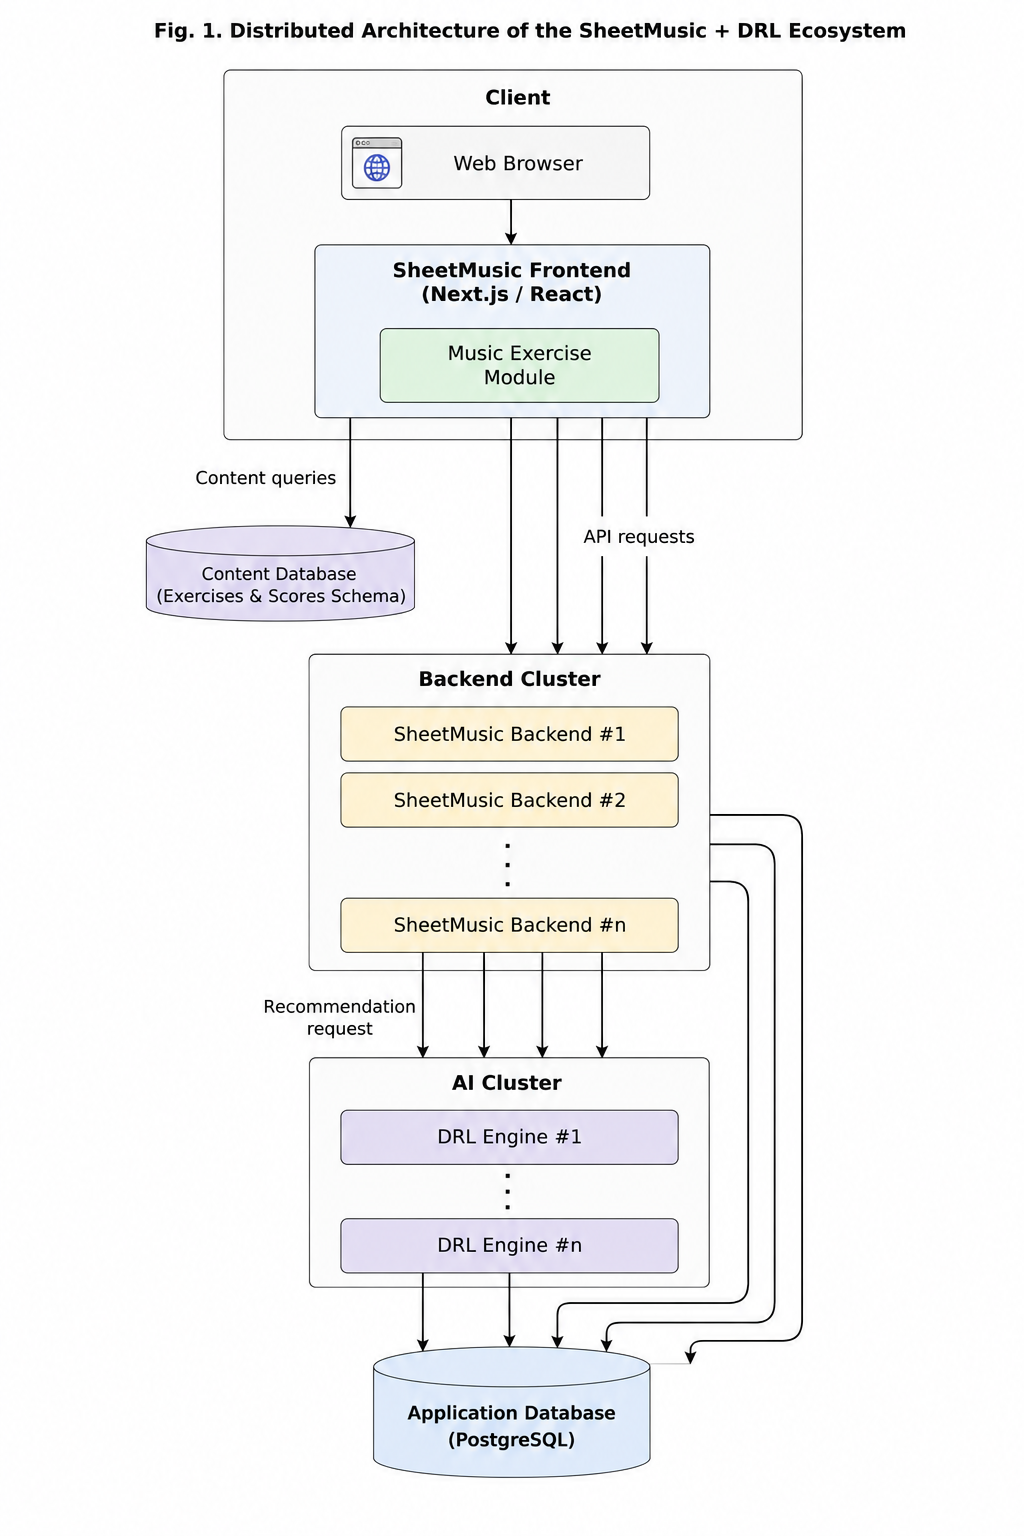
\includegraphics[width=0.48\textwidth]{Imagenes/fig_arch_system.png}}
\caption{Diagrama de arquitectura distribuida del ecosistema SheetMusic + DRL.}
\label{fig_arch}
\end{figure}
